\documentclass[11pt]{article}

% --- Silnik: xelatex ---
\usepackage{fontspec}
\setmainfont{TeX Gyre Pagella}
\setsansfont{TeX Gyre Heros}[Scale=0.92]
\setmonofont{TeX Gyre Cursor}[Scale=0.90]

\usepackage{amsmath}
\usepackage{amssymb}
\usepackage[a4paper,margin=2.4cm]{geometry}
\usepackage{xcolor}
\usepackage{titlesec}
\usepackage{enumitem}
\usepackage{booktabs}
\usepackage{tabularx}
\usepackage{array}
\usepackage{tikz}
\usetikzlibrary{automata,positioning,arrows.meta,fit,backgrounds,calc,shapes.geometric}
\usepackage[european,RPvoltages]{circuitikz}
\usepackage{graphicx}
\usepackage[section]{placeins}
\usepackage{caption}
\usepackage[hidelinks]{hyperref}

\definecolor{navy}{RGB}{0,0,0}
\definecolor{rulegrey}{RGB}{180,190,205}
\definecolor{accent}{RGB}{0,110,90}

\emergencystretch=3em
\hbadness=2500

\renewcommand{\figurename}{Rys.}
\renewcommand{\tablename}{Tab.}
\renewcommand{\contentsname}{Spis treści}
\captionsetup{font=it,labelfont=it,labelsep=period,width=0.92\linewidth}

\titleformat{\section}{\Large\bfseries\sffamily\color{navy}}{\thesection.}{0.5em}{}
\titleformat{\subsection}{\large\bfseries\sffamily\color{navy}}{\thesubsection.}{0.5em}{}
\titleformat{\subsubsection}{\normalsize\bfseries\sffamily\color{navy}}{\thesubsubsection.}{0.5em}{}
\titlespacing*{\section}{0pt}{1.25em}{0.45em}
\titlespacing*{\subsection}{0pt}{0.85em}{0.2em}
\titlespacing*{\subsubsection}{0pt}{0.6em}{0.15em}

\setlength{\parindent}{0pt}
\setlength{\parskip}{0.5em}
\setlist[itemize]{leftmargin=1.35em,itemsep=0.18em,topsep=0.25em}
\setlist[enumerate]{leftmargin=1.6em,itemsep=0.18em,topsep=0.25em}

\newcommand{\key}[1]{#1}

\begin{document}

% ====== TYTUL ======
\begin{center}
{\sffamily\bfseries\color{navy}\LARGE Stanowisko diagnostyczne ładowarek AC}\\[4pt]
{\sffamily\large\color{navy} Cyfrowy bliźniak EVSE i symulator pojazdu --- projekt własny}\\[7pt]
{\color{rulegrey}\rule{0.85\linewidth}{1pt}}\\[5pt]
{\sffamily\small Dawid Cekała \quad$\cdot$\quad zadanie rekrutacyjne AMPERE POINT (część 2) \quad$\cdot$\quad 19 czerwca 2026}
\end{center}

\vspace{0.4em}

\noindent\textbf{Streszczenie.} Przedmiotem projektu jest stanowisko, które bada ładowarkę AC do pojazdów elektrycznych od zewnątrz: automatycznie, powtarzalnie i bez prawdziwego samochodu. Ponieważ oprogramowanie ładowarki jest zamknięte, jej poprawne zachowanie opisuję jako model odniesienia zgodny z normą IEC 61851 (tak zwany złoty wzorzec) i sprawdzam, gdzie rzeczywista ładowarka od niego odbiega. Stanowisko składa się z symulatora pojazdu, modelu wzorcowego ładowarki, warstwy fizycznej linii sygnałowej oraz toru mocy z licznikiem energii; uzupełnia je mechanizm wstrzykiwania usterek i komparator wystawiający wynik wraz z raportem dla producenta. Stanowisko działa w symulacji (MATLAB/Simulink/Simscape), bez nakładów sprzętowych, ze ścieżką do wersji sprzętowej. Dokument przedstawia definicję problemu, założenia, logikę działania, możliwość rzeczywistej implementacji, budżet oraz ocenę wykonalności samodzielnej.

\vspace{0.2em}
{\color{rulegrey}\rule{\linewidth}{0.6pt}}

\tableofcontents
\newpage

% ==========================================================
\section{Sformułowanie problemu}

\subsection{Kontekst}

AMPERE POINT dostarcza inteligentne ładowarki AC do pojazdów elektrycznych (EV, ang.\ \textit{electric vehicle}): naścienne (wallbox) o mocy 11 i 22~kW oraz przenośne. Firma działa w modelu, w którym sprowadza gotowy sprzęt od producenta, testuje go, wdraża i sprzedaje bezpośrednio. Oprogramowanie układowe (firmware) pochodzi od producenta i jest zamknięte --- firma nie zmienia kodu, lecz zgłasza uwagi i otrzymuje poprawione wersje. Z punktu widzenia serwisu czarną skrzynką jest przede wszystkim firmware ładowarki: znane są jej wejścia i wyjścia, ale nie kod, który nimi steruje.

Firma świadomie rezygnuje z protokołu OCPP (ang.\ \textit{Open Charge Point Protocol} --- otwarty protokół łączący stację ładowania z systemem zarządzania), stawiając na prosty sprzęt z niezerowalnym licznikiem energii. Licznik służy do rozliczania kosztów ładowania w małych flotach: pracownik ładuje auto służbowe, a firma rozlicza koszt na podstawie odczytu. Dokładność licznika jest więc nie detalem, lecz realną wartością biznesową.

\subsection{Problem do rozwiązania}

Serwis i kontrola jakości takiej ładowarki napotykają trzy trudności.

\begin{itemize}
  \item \key{Potrzeba samochodu.} Żeby sprawdzić ładowarkę, trzeba podłączyć do niej pojazd. Samochód jest drogi, zajmuje miejsce, reaguje tylko w sposób przewidziany przez producenta i trudno wymusić na nim zachowania brzegowe. Nie da się go też zautomatyzować do powtarzalnego testu.
  \item \key{Regresje firmware.} Producent co jakiś czas przysyła nowy firmware, który może naprawić jedną rzecz, a zepsuć inną. Bez powtarzalnego testu taką regresję trudno wychwycić, zanim sprzęt trafi do klienta.
  \item \key{Niejasne zgłoszenia.} Gdy z terenu przychodzi zgłoszenie „nie działa”, trudno je odtworzyć i zamienić w konkretny, mierzalny opis dla producenta.
\end{itemize}

Narzędzie, które firma dziś rozdaje klientom --- podstawowy tester wallboxów --- odpowiada jedynie na pytanie \key{„czy w ogóle działa”} (wynik typu tak/nie). Nie odpowiada na pytanie \key{„jak dokładnie się zachowuje, gdzie odbiega od normy i o ile”}.

\subsection{Cel i zakres}

Celem projektu jest stanowisko, które bada ładowarkę AC \key{od zewnątrz}: automatycznie, powtarzalnie i bez prawdziwego samochodu. Ponieważ nie dysponujemy kodem ładowarki, opisujemy jej poprawne zachowanie jako \key{model odniesienia} zgodny z normą IEC 61851 (norma definiująca przewodowe ładowanie pojazdów elektrycznych) i sprawdzamy, gdzie rzeczywista ładowarka od tego modelu odbiega.

Stanowisko emuluje stronę pojazdu, prowadzi ładowarkę przez kolejne stany ładowania, mierzy jej odpowiedzi, wstrzykuje wybrane usterki i wystawia wynik wraz z raportem nadającym się do przesłania producentowi. Działa w symulacji, bez nakładów sprzętowych; ścieżkę do wersji sprzętowej opisano w rozdziale~\ref{sec:impl}.

% ==========================================================
\section{Założenia projektowe}\label{sec:zal}

Założenia spinają cały projekt; do nich odwołują się później decyzje techniczne i ocena wykonalności.

\begin{enumerate}
  \item \key{Tylko ładowanie prądem przemiennym.} Zakres obejmuje ładowanie AC w standardzie gniazda Type~2, jedno- i trójfazowe, z podstawową komunikacją wg IEC 61851 (sygnał PWM na linii Control Pilot). Świadomie poza zakresem pozostają ISO 15118 i komunikacja po linii zasilającej (PLC, ang.\ \textit{Power Line Communication}) oraz OCPP --- zgodnie z profilem produktu firmy.
  \item \key{Ładowarka jako czarna skrzynka.} Nie modelujemy kodu ładowarki, lecz jej poprawne zachowanie wynikające z normy. Model jest odniesieniem, do którego porównujemy obiekt badany, a nie kopią firmware.
  \item \key{Bezpieczeństwo w pierwszej kolejności.} Stanowisko pracuje po stronie niskonapięciowej sygnalizacji (linie Control Pilot i Proximity Pilot). Tor mocy 230/400~V jest modelowany w symulacji; pobór rzeczywistego prądu to osobny krok sprzętowy z właściwymi zabezpieczeniami.
  \item \key{Narzędzie wspomagające, nie certyfikujące.} Stanowisko uzupełnia, a nie zastępuje, certyfikowane mierniki bezpieczeństwa. Służy diagnostyce i kontroli jakości, nie formalnej certyfikacji.
  \item \key{Kapitał bliski zera.} Najpierw model i symulacja (MATLAB/Simulink/Simscape lub darmowe odpowiedniki), dopiero potem ewentualny sprzęt. Odpowiada to strategii firmy, by nie angażować kapitału w przedwczesne prototypy.
  \item \key{Powtarzalność i automatyzacja.} Każdy test daje ten sam wynik przy tych samych warunkach i nadaje się do uruchomienia w serii, co umożliwia regresję po każdym nowym firmware.
\end{enumerate}

% ==========================================================
\section{Użyteczność}

Stanowisko jest świadomym rozwinięciem testera, który firma już dziś rozdaje --- od odpowiedzi „świeci się / nie świeci” do realnej diagnostyki i kontroli jakości. Adresaci i zastosowania:

\begin{itemize}
  \item \key{Serwisant} --- odtworzenie zgłoszenia z terenu w warunkach laboratoryjnych, bez podłączania samochodu, i wskazanie, w której warstwie tkwi usterka.
  \item \key{Kontrola jakości} --- sprawdzenie partii ze sprawdzeniem licznika energii i czasów reakcji, zanim sprzęt trafi do klienta.
  \item \key{Regresja firmware} --- automatyczne przejście całego zestawu testów po każdej nowej wersji oprogramowania, z porównaniem do poprzedniej.
  \item \key{Materiał dla producenta} --- zamiana mglistego „nie działa” w konkretny raport: który scenariusz, jaka odchyłka, o ile i jak ją odtworzyć. To skraca pętlę poprawek z fabryką.
  \item \key{Ochrona rozliczeń flotowych} --- weryfikacja, że licznik energii nie zawyża i nie zaniża odczytu, czyli że faktury dla floty są poprawne.
\end{itemize}

% ==========================================================
\section{Niezbędne podstawy techniczne}

Krótki fundament, bez którego logika stanowiska nie miałaby sensu.

\subsection{Ładowarka AC to inteligentny włącznik, nie prostownik}

Bateria pojazdu przyjmuje prąd stały (DC, ang.\ \textit{direct current}), a z sieci płynie prąd przemienny (AC, ang.\ \textit{alternating current}). Zamianę AC na DC, czyli prostowanie, wykonuje prostownik znajdujący się \key{w samochodzie} (ładowarka pokładowa). Ładowarka AC --- wallbox lub stacja przenośna --- nie zamienia prądu: podaje do auta prąd przemienny, uzgadnia z nim dopuszczalną wartość prądu oraz załącza i odłącza zasilanie. Cała jej „inteligencja” sprowadza się do sygnalizacji, sterowania i zabezpieczeń --- i właśnie to można modelować oraz badać od zewnątrz. W normach taką ładowarkę określa skrót EVSE (ang.\ \textit{Electric Vehicle Supply Equipment} --- sprzęt zasilający pojazd elektryczny).

\subsection{Control Pilot i stany ładowania}

Komunikacja idzie jedną żyłą sygnałową, zwaną Control Pilot (CP). Ładowarka podaje na nią napięcie, a samochód swoimi rezystorami obniża je do określonych poziomów; każdy poziom oznacza inny stan (Tab.~\ref{tab:stany}). Gdy auto jest gotowe, ładowarka nadaje na CP sygnał prostokątny o częstotliwości 1~kHz (PWM, ang.\ \textit{pulse-width modulation} --- modulacja szerokości impulsu), którego wypełnienie koduje dopuszczalny prąd. Całą tę wymianę nazywa się sekwencją uzgadniania (handshake).

\begin{table}[h]
\centering
\begin{tabularx}{0.9\linewidth}{@{}c c X@{}}
\toprule
\textbf{Stan} & \textbf{Napięcie CP} & \textbf{Znaczenie} \\
\midrule
A & $+12$~V & brak pojazdu (spoczynek) \\
B & $+9$~V & pojazd podłączony, jeszcze nie ładuje \\
C & $+6$~V & pojazd ładuje \\
D & $+3$~V & ładowanie z wymuszoną wentylacją (rzadkie) \\
E / F & $0$ / $-12$~V & błąd / ładowarka niedostępna \\
\bottomrule
\end{tabularx}
\caption{Stany linii Control Pilot i odpowiadające im poziomy napięcia.}
\label{tab:stany}
\end{table}

W zbudowanym obwodzie CP poziomy wynoszą 12,00~V (stan~A), 8,98~V (stan~B) i 5,99~V (stan~C), co potwierdza dobór rezystorów opisany w punkcie~\ref{sec:cp}.

\subsection{Kodowanie prądu i Proximity Pilot}

Dopuszczalny prąd wynika wprost z wypełnienia sygnału: \key{prąd [A] = wypełnienie [\%] $\times$ 0,6}, w zakresie 10--85\%. Na przykład 25\% odpowiada 15~A, 50\% odpowiada 30~A, a około 53\% odpowiada 32~A. Druga żyła, Proximity Pilot (PP), koduje rezystorem rodzaj kabla i jego obciążalność (na przykład 1,5~k$\Omega$ to 13~A, 680~$\Omega$ to 20~A, 220~$\Omega$ to 32~A). Ładowarka nigdy nie oferuje prądu większego, niż wytrzyma kabel.

\subsection{Licznik energii i równoważenie mocy}

Ładowarki mają niezerowalny licznik energii (kWh), będący podstawą rozliczeń flotowych. Funkcja dynamicznego równoważenia obciążenia (DLB, ang.\ \textit{Dynamic Load Balancing}) rozdziela dostępną moc między stacje tak, by suma prądów nie przekroczyła prądu znamionowego bezpiecznika instalacji: gdy w budynku rośnie inne obciążenie, ładowarka musi w porę zmniejszyć prąd, a po odłączeniu auta zwiększyć go ponownie. Zabezpieczenie różnicowoprądowe (RCD, ang.\ \textit{residual current device}) typu~A z detekcją 6~mA prądu stałego chroni przed porażeniem. Te dwa obszary --- dokładność licznika i poprawność równoważenia mocy --- to najczęstsze miejsca realnych problemów.

% ==========================================================
\section{Architektura i logika działania}

\subsection{Ogólna architektura}

Architektura obejmuje sześć współpracujących części. Zbudowany rdzeń (Rys.~\ref{rys:arch}) zawiera cztery z nich: symulator pojazdu i wzorzec ładowarki (dwie maszyny stanów), które spotykają się na wspólnej \key{warstwie fizycznej Control Pilot} pełniącej rolę kabla oraz osobno na \key{torze mocy} z licznikiem; spina je logika stycznika. Pozostałe dwie części --- sekwencer scenariuszy z wstrzykiwaniem usterek oraz komparator z generatorem raportu --- to warstwa nadbudowywana nad tym rdzeniem: sekwencer ustawia scenariusz i usterki, a komparator porównuje zachowanie obiektu badanego z wzorcem (oraz z wartościami oczekiwanymi z normy) i wystawia wynik wraz z raportem.

\begin{figure}[ht]
\centering
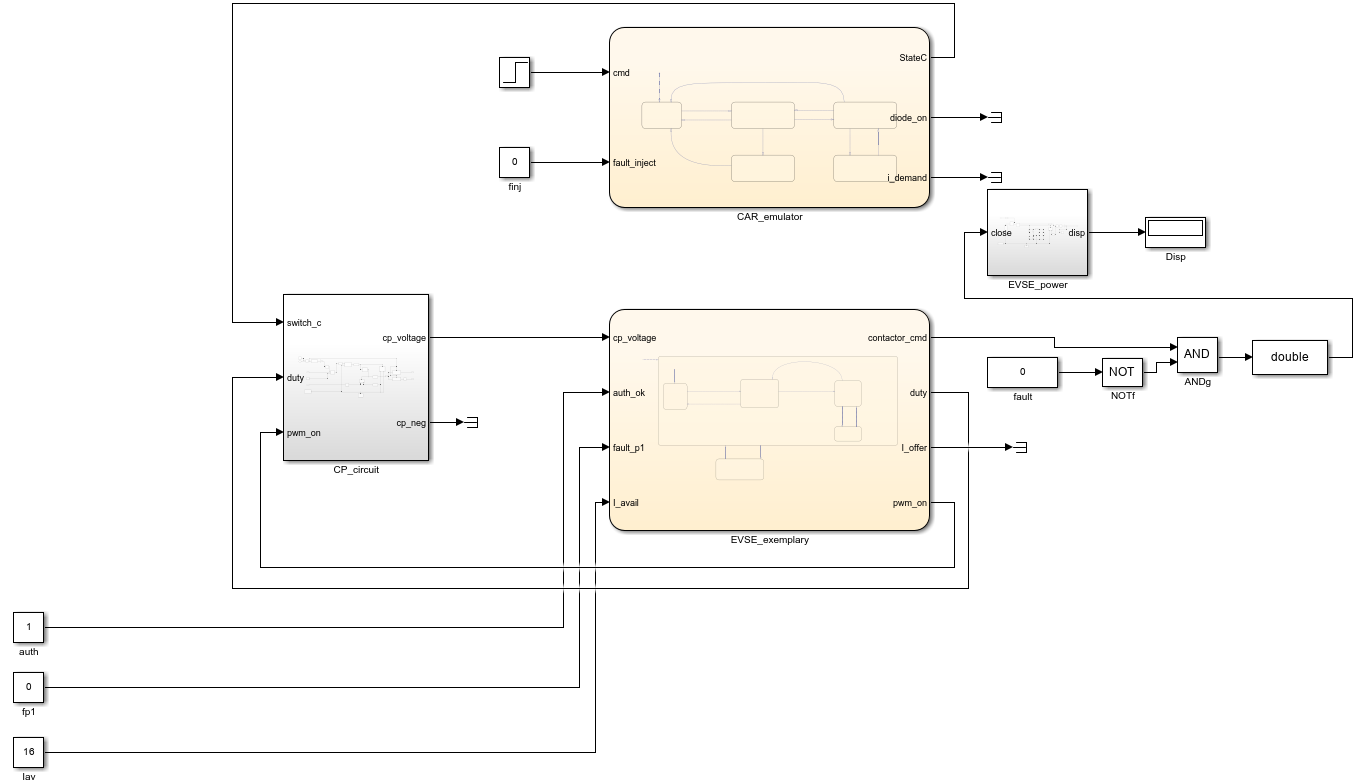
\includegraphics[width=\linewidth]{schemat_model.png}
\caption{Zbudowany model w~Simulink: emulator pojazdu i~wzorzec ładowarki (karty Stateflow, żółte) oraz obwód Control Pilot i~tor mocy z~licznikiem (podsystemy Simscape), spięte logiką stycznika. Komparator i~raport to warstwa nadbudowywana nad tym rdzeniem.}
\label{rys:arch}
\end{figure}

\begin{table}[h]
\centering
\begin{tabularx}{\linewidth}{@{}l c X@{}}
\toprule
\textbf{Sygnał} & \textbf{Jedn.} & \textbf{Znaczenie} \\
\midrule
\texttt{cp\_voltage} & V & napięcie linii Control Pilot, czytane przez wzorzec \\
\texttt{duty} & \% & wypełnienie PWM kodujące oferowany prąd \\
\texttt{StateC} & 0/1 & polecenie pojazdu „jestem gotów” (przejście B$\to$C) \\
\texttt{i\_demand} & A & prąd, jaki pojazd chce pobrać \\
\texttt{I\_offer} & A & prąd oferowany przez ładowarkę \\
\texttt{contactor\_cmd} & 0/1 & polecenie zamknięcia stycznika mocy \\
\texttt{E\_true / E\_meter} & kWh & energia rzeczywista / zliczona przez licznik \\
\texttt{verdict} & --- & wynik testu wraz z odchyłką \\
\bottomrule
\end{tabularx}
\caption{Sygnały wymieniane między częściami modelu.}
\label{tab:sygnaly}
\end{table}

\subsection{Trzy zagnieżdżone pętle sterowania}

Wnętrze ładowarki --- a więc i wzorca --- porządkują trzy zagnieżdżone pętle (Rys.~\ref{rys:petle}); to standard oprogramowania EVSE.

\begin{itemize}
  \item \key{Pętla 1 --- bezpieczeństwo} (czas rzędu milisekund). Generacja i odczyt sygnału CP, zabezpieczenia (RCD, monitoring przewodu ochronnego PE, wykrycie sklejonego stycznika, nadprąd) oraz wykonawcze sterowanie stycznikiem. Działa odruchowo: usterka powoduje natychmiastowe otwarcie stycznika.
  \item \key{Pętla 2 --- sterowanie} (dziesiątki milisekund do sekund). Maszyna stanów uzgadniania A--B--C, decyzja o wypełnieniu PWM (czyli o oferowanym prądzie), zarządzanie sesją i równoważenie mocy DLB.
  \item \key{Pętla 3 --- aplikacja}. Łączność, autoryzacja RFID, licznik energii, harmonogramy. Ustawia nastawy dla pętli 2, ale sama nie dotyka stycznika.
\end{itemize}

Warstwa wyższa zadaje cele niższej, lecz pętla bezpieczeństwa może zawsze przebić pozostałe. Ten podział ma wartość diagnostyczną: usterka, na którą stycznik nie reaguje, wskazuje na pętlę~1; zły prąd przy zamkniętym styczniku --- na pętlę~2; przekłamanie licznika --- na pętlę~3.

\begin{figure}[h]
\centering
\begin{tikzpicture}[font=\sffamily\small]
 \draw[rounded corners,thick,draw=navy,fill=navy!4] (0,0) rectangle (13,6.3);
 \node[anchor=north west,navy,font=\sffamily\bfseries\footnotesize] at (0.25,6.15) {Pętla 3 --- aplikacja (łączność/chmura, RFID, licznik kWh, harmonogramy)};
 \draw[rounded corners,thick,draw=navy,fill=navy!9] (0.7,0.6) rectangle (12.3,4.8);
 \node[anchor=north west,navy,font=\sffamily\bfseries\footnotesize] at (0.95,4.65) {Pętla 2 --- sterowanie (handshake IEC 61851, PWM = prąd, DLB)};
 \draw[rounded corners,thick,draw=navy,fill=navy!16] (1.45,1.2) rectangle (11.55,3.3);
 \node[anchor=north west,navy,font=\sffamily\bfseries\footnotesize] at (1.7,3.15) {Pętla 1 --- bezpieczeństwo (RCD, PE, stan E/F)};
 \node[align=center,font=\sffamily\footnotesize,navy] at (6.5,1.95) {odruchowe, nadrzędne\\weto nad stycznikiem};
\end{tikzpicture}
\caption{Trzy zagnieżdżone pętle sterowania. Warstwa wyższa zadaje cele niższej; pętla bezpieczeństwa może w każdej chwili przebić pozostałe.}
\label{rys:petle}
\end{figure}

\subsection{Logika stycznika: pozwolenie i nadrzędne weto}\label{sec:contactor}

Stycznik mocy jest jeden, ale dwie pętle mają nad nim władzę o różnym charakterze. W normalnej pracy załącza go i wyłącza pętla~2: po poprawnym przejściu do stanu~C zamyka obwód, a po zakończeniu sesji go otwiera. Pętla~1 ma prawo nadrzędnego weta --- otwiera stycznik niezależnie od pętli~2, gdy wykryje usterkę. Regułę zapisuje jeden warunek:
\[
\text{stycznik zamknięty} = (\text{pętla 2 każe zamknąć}) \;\wedge\; \lnot(\text{pętla 1 zgłasza usterkę}).
\]
W modelu odpowiada temu bramka logiczna sterująca przełącznikiem toru mocy: zamknięcie następuje, gdy \texttt{contactor\_cmd} jest aktywne i jednocześnie nie ma usterki. Załączyć moc może tylko pętla sterująca i tylko wtedy, gdy pętla bezpieczeństwa na to pozwala; otworzyć stycznik może każda z nich, a otwarcie z pętli bezpieczeństwa jest nadrzędne.

\subsection{Warstwa fizyczna Control Pilot}\label{sec:cp}

Obwód Control Pilot (Rys.~\ref{rys:cp}) odtwarza realne napięcia linii, dzięki czemu na wykresie widać warstwę fizyczną, a nie tylko liczby. Po stronie ładowarki źródło podaje na linię $\pm$12~V --- w spoczynku stałe $+12$~V, a podczas oferowania prądu sygnał PWM --- a rezystor $R_1=1$~k$\Omega$ tworzy z siecią rezystorów pojazdu dzielnik napięcia. Po stronie pojazdu dioda i rezystor $R_2=2{,}74$~k$\Omega$ ustalają w stanie~B poziom około 9~V; dioda jest po to, by ładowarka rozpoznała prawdziwy pojazd, bo rezystor bez diody traktuje jako usterkę. Dla stanu~C symulator pojazdu dołącza równolegle rezystor $R_3=1{,}3$~k$\Omega$ przez przełącznik, co obniża poziom do około 6~V. Woltomierz mierzy napięcie węzła CP i przekazuje je obu maszynom stanów.

Wartości progów wynikają wprost z dzielnika. Dla stanu~B napięcie wynosi $12\cdot 2{,}74/(1+2{,}74)\approx 9$~V. Po dołączeniu $R_3$ równolegle opór pojazdu maleje do około 0,88~k$\Omega$, a napięcie do około 6~V (stan~C). Zbudowany model daje odpowiednio 8,98~V i 5,99~V, co potwierdza dobór elementów.

Napięcie pilota powstaje w modelu z dwóch sygnałów wzorca: \texttt{pwm\_on} decyduje, czy linia jest stała czy migająca, a \texttt{duty} ustala szerokość impulsu. Ponieważ sygnał oscyluje, pomiar jest próbkowany w~rytm PWM: próbka z górnej części fali daje stabilny poziom stanu (\texttt{cp\_voltage}), a z dolnej --- kontrolę obecności diody (\texttt{cp\_neg}).

\begin{figure}[ht]
\centering
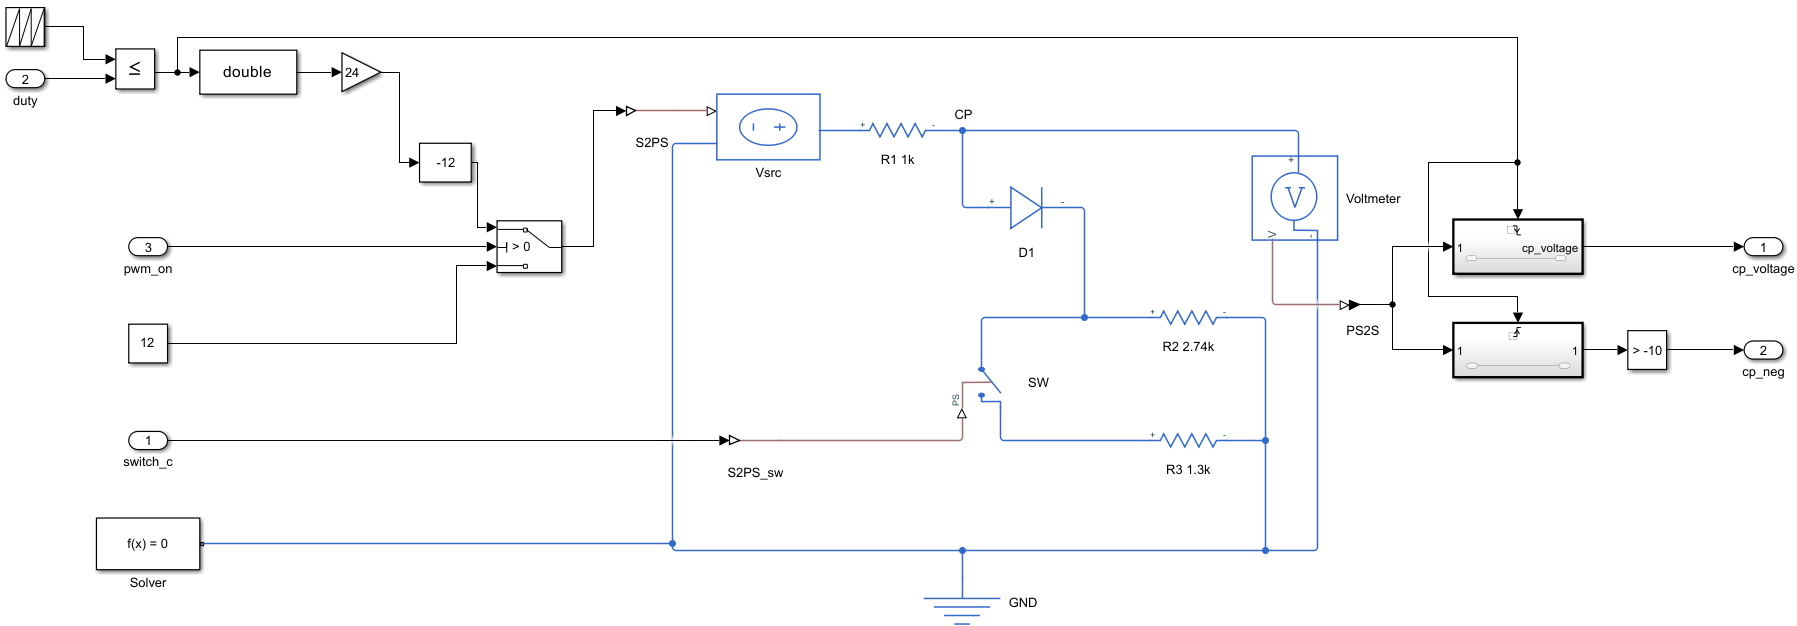
\includegraphics[width=\linewidth]{schemat_cp.png}
\caption{Obwód Control Pilot (podsystem). Po lewej generator sygnału: piła 1~kHz, porównanie z~wypełnieniem i~przełącznik trybu dają na źródle Vsrc stałe $+12$~V albo falę $\pm$12~V. W~środku dzielnik z~diodą ($R_1$, $R_2$, $R_3$, SW) ustalający poziomy 12/9/6~V. Po prawej próbkowanie szczytów: \texttt{cp\_voltage} (poziom stanu) oraz \texttt{cp\_neg} (kontrola diody).}
\label{rys:cp}
\end{figure}

\subsection{Maszyny stanów}

Dwie karty Stateflow stanowią serce logiki: jedna udaje pojazd, druga jest wzorcem ładowarki. Dogadują się one przez fizyczny węzeł CP, a nie przez sztywno połączony sygnał --- i to czyni model wiernym cyfrowym bliźniakiem.

Symulator pojazdu (Rys.~\ref{rys:emul}) przechodzi stany od A (odłączony), przez B (podłączony), do C (gotów do ładowania), z dodatkową gałęzią Fault. Jego wyjścia określają, które rezystory i diodę wpiąć w obwód CP oraz ile prądu pojazd chce pobrać; wejściem są komendy ze sekwencera.

\begin{figure}[ht]
\centering
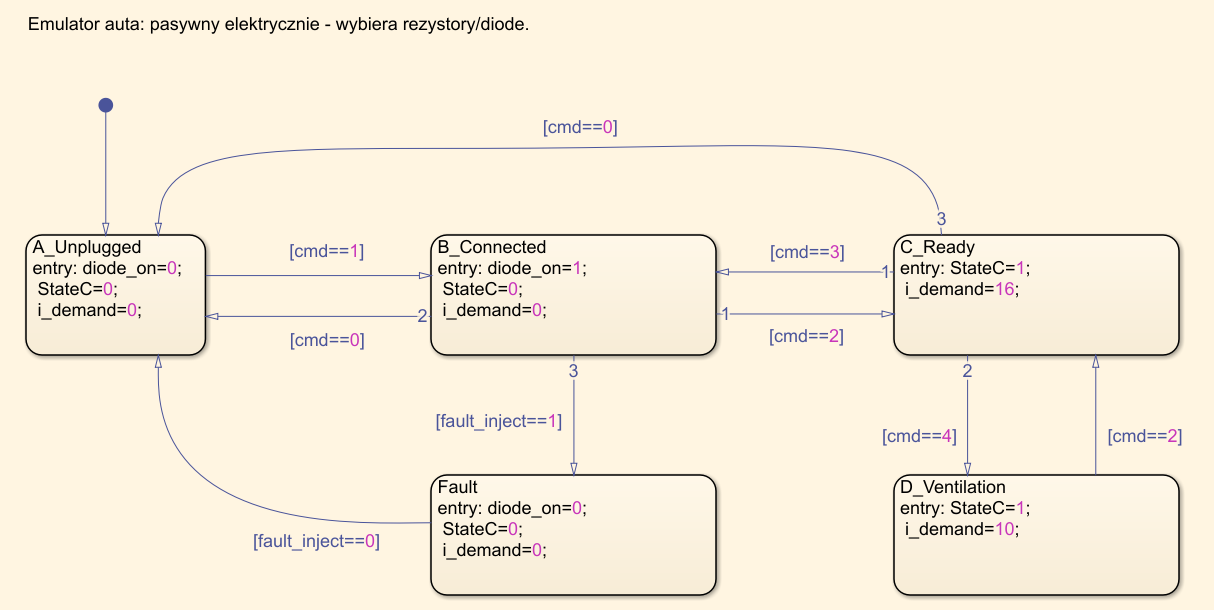
\includegraphics[width=\linewidth]{schemat_emulator.png}
\caption{Maszyna stanów symulatora pojazdu (Stateflow). Od stanu A (odłączony) przez B i~C do~D, z~gałęzią Fault; wyjścia \texttt{StateC}, \texttt{diode\_on} i~\texttt{i\_demand} sterują stroną pojazdu.}
\label{rys:emul}
\end{figure}

Wzorzec ładowarki (Rys.~\ref{rys:evse}) czyta napięcie CP, wnioskuje z niego stan pojazdu i reaguje zgodnie z normą. W stanie Idle utrzymuje stałe $+12$~V; po wykryciu 9~V włącza PWM o wypełnieniu odpowiadającym prądowi (stan Detected); po wykryciu 6~V zamyka stycznik i rozpoczyna ładowanie (Charging); przy napięciu niedozwolonym przechodzi w stan Tripped i otwiera stycznik. Wszystkie stany pracy obejmuje nadrzędna gałąź bezpieczeństwa, zgodna z regułą stycznika z punktu~\ref{sec:contactor}.

\begin{figure}[ht]
\centering
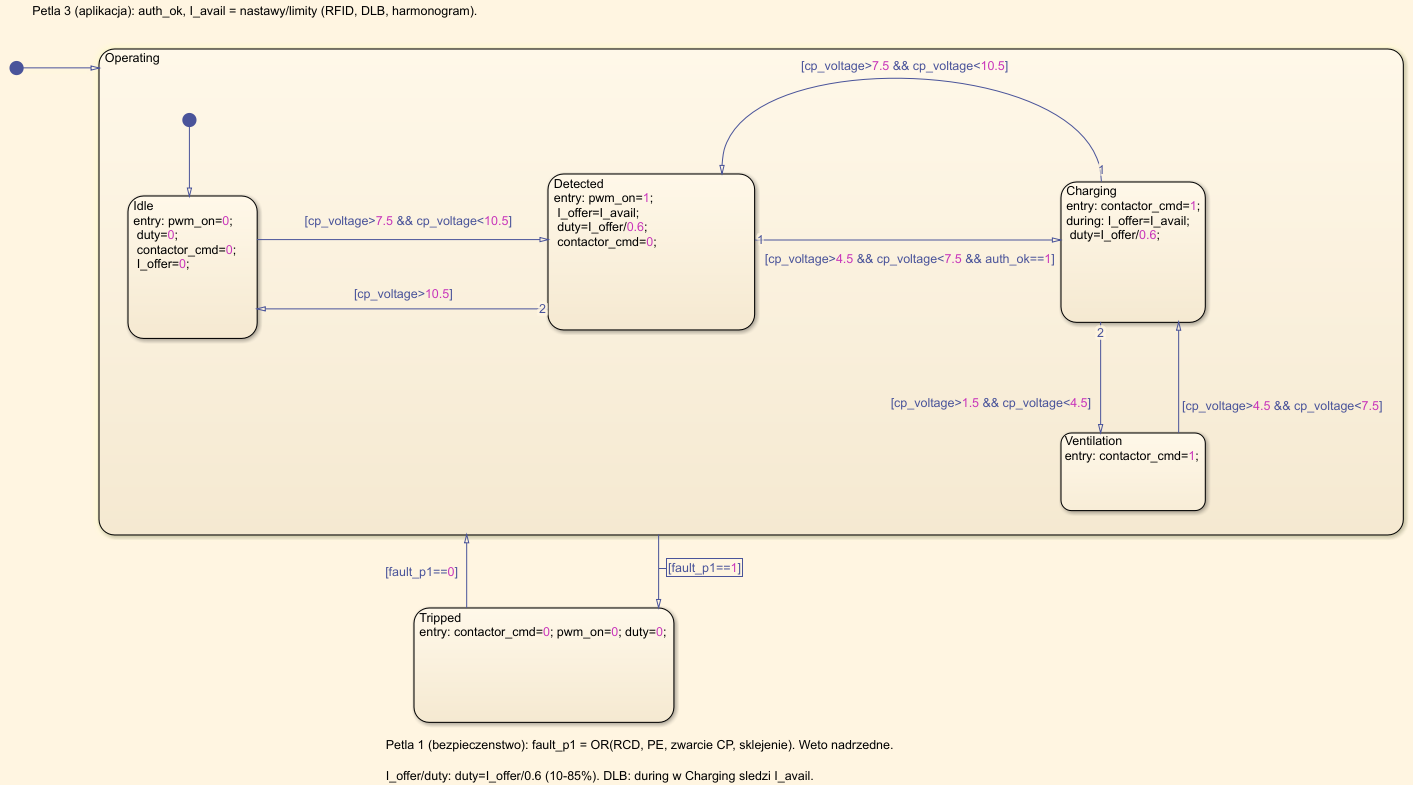
\includegraphics[width=\linewidth]{schemat_wzorzec.png}
\caption{Maszyna stanów wzorca ładowarki (Stateflow). Grupa Operating (Idle, Detected, Charging, Ventilation) prowadzi handshake według poziomu CP; nadrzędny stan Tripped odpowiada wetu pętli bezpieczeństwa (\texttt{fault\_p1}).}
\label{rys:evse}
\end{figure}

\subsection{Tor mocy i licznik energii}

Tor mocy (Rys.~\ref{rys:moc}) sprawdza, czy zliczona energia zgadza się z prawdą --- a to filar rozliczeń flotowych. Źródło prądu przemiennego (230/400~V) zasila obwód przez stycznik sterowany regułą z punktu~\ref{sec:contactor}. Czujniki prądu i napięcia mierzą wielkości na wejściu odbiornika, którym jest model ładowarki pokładowej pojazdu: mostek prostowniczy, kondensator wygładzający i bateria. Iloczyn napięcia i prądu daje moc chwilową, a jej całka po czasie --- energię rzeczywistą $E_\text{true}$ w kWh. Ten sam przebieg, przepuszczony przez konfigurowalny błąd licznika (offset, dryf, kwantyzacja), daje wartość zliczoną $E_\text{meter}$. Komparator liczy błąd procentowy i porównuje go z tolerancją.

Warto zaznaczyć, że licznik mierzy energię po stronie prądu przemiennego --- i tak właśnie robi prawdziwa ładowarka, bo to tę energię się rozlicza. Prostowanie z prądu przemiennego na stały zachodzi w tym odbiorniku reprezentującym auto, czyli już za licznikiem.

\begin{figure}[ht]
\centering
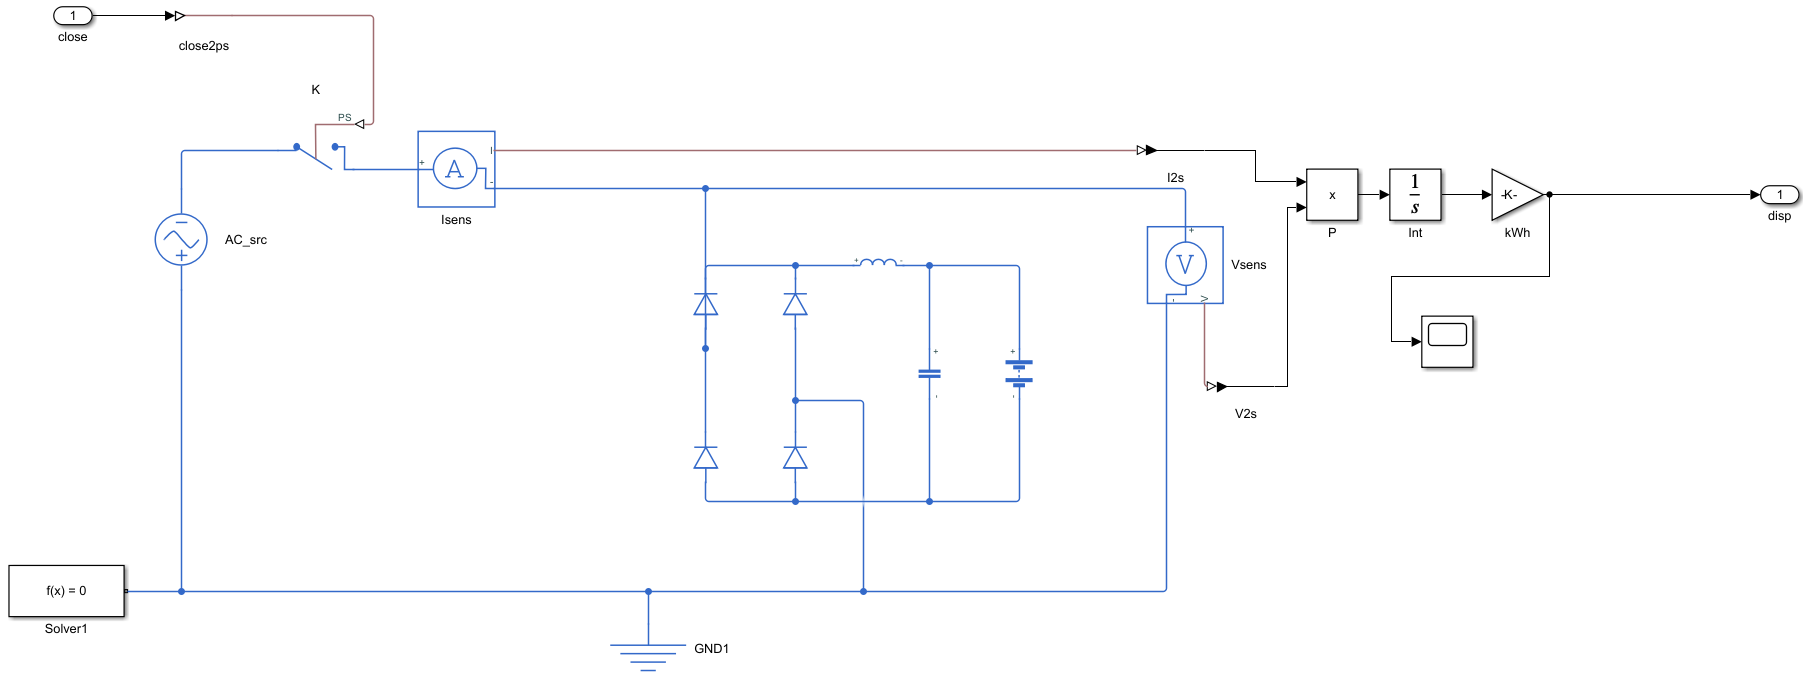
\includegraphics[width=\linewidth]{schemat_tor_mocy.png}
\caption{Tor mocy (podsystem). Źródło AC zasila przez stycznik $K$ i~czujnik prądu mostek prostowniczy z~dławikiem, kondensatorem i~baterią --- model ładowarki pokładowej pojazdu. Iloczyn napięcia i~prądu, scałkowany w~czasie, daje energię w~kWh.}
\label{rys:moc}
\end{figure}

\subsection{Wstrzykiwanie usterek i komparator}

Sekwencer celowo psuje model przełącznikami i flagami, odtwarzając realne awarie (Tab.~\ref{tab:usterki}). Komparator porównuje obiekt badany z wzorcem: różnicę prądu z tolerancją, czas reakcji z progiem, błąd licznika z dopuszczalnym oraz legalność przejść stanów. Wynikiem jest werdykt pozytywny lub negatywny (pass/fail) wraz ze zmierzoną odchyłką, z którego sekwencer buduje raport dla producenta.

\begin{table}[h]
\centering
\begin{tabularx}{\linewidth}{@{}l X X@{}}
\toprule
\textbf{Usterka} & \textbf{Co psuje} & \textbf{Oczekiwana reakcja wzorca} \\
\midrule
\texttt{no\_diode} & wyłącza diodę pojazdu & wykrycie i odmowa ładowania \\
\texttt{cp\_short} & wymusza 0~V na linii CP & przejście w stan E (błąd) \\
\texttt{duty\_error} & przesuwa wypełnienie PWM & sygnalizacja złego prądu oferowanego \\
\texttt{slow\_response} & opóźnia zmianę wypełnienia & wykrycie zbyt wolnej reakcji DLB \\
\texttt{meter\_error} & dodaje błąd do licznika & wykrycie odchyłki kWh ponad tolerancję \\
\bottomrule
\end{tabularx}
\caption{Katalog wstrzykiwanych usterek i oczekiwanej reakcji modelu wzorcowego.}
\label{tab:usterki}
\end{table}

% ==========================================================
\section{Scenariusze testowe}

Stanowisko realizuje zestaw scenariuszy. Dwa są kluczowe, trzeci spina je w proces.

\subsection{Scenariusz A --- weryfikacja licznika energii}

Zadaję znany profil prądu w sesji ładowania, liczę energię rzeczywistą jako całkę mocy po czasie i obarczam model licznika konfigurowalnym błędem. Stanowisko sygnalizuje, gdy zliczona wartość kWh odbiega od prawdy ponad przyjętą tolerancję (na przykład $\pm$1\%). Dzięki temu zanim sprzęt trafi do floty, wiadomo, czy licznik nie zawyża faktur, a jeśli zawyża --- znana jest dokładna wartość do zgłoszenia producentowi.

\subsection{Scenariusz B --- równoważenie mocy}

Modeluję instalację domową: bezpiecznik główny, zmienne obciążenie oraz od jednej do czterech ładowarek z funkcją DLB. Podnoszę obciążenie i sprawdzam dwie rzeczy: czy suma prądów nigdy nie przekracza prądu znamionowego bezpiecznika oraz czy ładowarka zdążyła zmniejszyć prąd w wymaganym czasie. Po odłączeniu auta sprawdzam, czy pozostałe stacje dobierają zwolnioną moc. Scenariusz wprost dotyka realnych skarg: zadziałania bezpiecznika lub niepotrzebnie wolnego ładowania.

\subsection{Regresja po nowym firmware}

Producent okresowo dostarcza nową wersję oprogramowania układowego, która może zmienić zachowanie ładowarki także poza obszarem, którego dotyczyła aktualizacja. Regresja polega na ponownym wykonaniu tego samego, ustalonego zestawu przypadków testowych na nowej wersji i zestawieniu wyników z wersją poprzednią oraz z wzorcem. Przypadek zakończony wcześniej wynikiem pozytywnym, a po aktualizacji negatywnym, oznacza regresję wprowadzoną przez nowy firmware. Ponieważ zestaw jest zautomatyzowany i powtarzalny, porównanie sprowadza się do różnicy dwóch zbiorów werdyktów i odchyłek, co ujawnia niezamierzone skutki uboczne aktualizacji przed wysyłką sprzętu do klienta.

% ==========================================================
\section{Możliwość rzeczywistej implementacji}\label{sec:impl}

Projekt jest pomyślany dwuetapowo, a każde założenie z rozdziału~\ref{sec:zal} ma tu odzwierciedlenie.

\subsection{Wariant symulacyjny}

Pierwszy etap jest w całości w oprogramowaniu. Zbudowano i zweryfikowano dotychczas: obwód Control Pilot z poprawnymi poziomami 9~V i 6~V, tor mocy z licznikiem energii oraz dwie maszyny stanów --- symulator pojazdu i wzorzec ładowarki. To dowód koncepcji bez nakładów i bez ryzyka, zgodny z założeniem „bezpieczeństwo w pierwszej kolejności” i „kapitał bliski zera”.

\subsection{Wariant sprzętowy --- adapter}

Drugi etap to tani adapter, który podłącza prawdziwą ładowarkę do tej samej logiki testowej. Kluczowa obserwacja: każdy blok-mostek w symulacji ma fizyczny odpowiednik w sprzęcie, więc \key{symulacja jest wprost specyfikacją adaptera} (Tab.~\ref{tab:hil}). Mikrokontroler (MCU, na przykład ESP32 lub STM32) obsługuje linie Control Pilot i Proximity Pilot gniazda Type~2: odczytuje wypełnienie sygnału ładowarki, przełącza rezystory i diodę po stronie pojazdu, koduje kabel rezystorem PP, a wyniki przesyła do komputera. Wzorzec pozostaje w oprogramowaniu jako odniesienie, a komparator i raport nie zmieniają się. Ponieważ napięcia sieci dotyka dopiero część mocy, ten krok wykonuje się z właściwymi zabezpieczeniami --- zgodnie z założeniem~3.

\begin{table}[h]
\centering
\begin{tabularx}{\linewidth}{@{}X X@{}}
\toprule
\textbf{Element symulacji} & \textbf{Odpowiednik sprzętowy} \\
\midrule
generator PWM + źródło CP & timer PWM mikrokontrolera + wzmacniacz do $\pm$12~V \\
czujnik napięcia CP & dzielnik z układem ograniczającym + przetwornik analogowo-cyfrowy (ADC) \\
przełącznik $R_3$ (stan C) & przekaźnik lub tranzystor MOSFET + rezystor \\
dioda pojazdu & dioda + przełącznik (do wstrzyknięcia usterki) \\
kodowanie Proximity Pilot & bank rezystorów (1,5~k$\Omega$ / 680~$\Omega$ / 220~$\Omega$) \\
stycznik toru mocy & izolowany detektor zamknięcia (tylko odczyt) \\
licznik energii & odczyt licznika ładowarki (wyjście impulsowe lub UART) \\
\bottomrule
\end{tabularx}
\caption{Most między symulacją a sprzętem: każdy blok-mostek modelu ma odpowiednik w peryferium mikrokontrolera i układzie pośredniczącym.}
\label{tab:hil}
\end{table}

\subsection{Wykonalność samodzielna i plan prac}

Projekt jest wykonalny samodzielnie. Twardy rdzeń obejmuje obwód CP, maszyny stanów, przeliczenie prądu i PP, wstrzykiwanie usterek z komparatorem, scenariusz licznika oraz raport (Tab.~\ref{tab:plan}); scenariusz równoważenia mocy jest rozszerzeniem realizowanym w dalszej kolejności. Kolejność prac jest „od dołu do góry”: najpierw działający obwód CP, potem kolejne warstwy, tak by po każdym kroku istniał działający i pokazywalny fragment, a nie wielki model, który nie chce ruszyć.

\begin{table}[h]
\centering
\begin{tabularx}{\linewidth}{@{}c X@{}}
\toprule
\textbf{Faza} & \textbf{Zakres} \\
\midrule
0 & Analiza normy IEC 61851 i lista przypadków testowych \\
1 & Warstwa fizyczna CP w Simscape (poziomy 12/9/6~V, PWM) \\
2 & Maszyny stanów: wzorzec ładowarki i symulator pojazdu \\
3 & Przeliczenie prądu, kodowanie PP, wartości raportowane \\
4 & Wstrzykiwanie usterek, komparator i werdykt \\
5 & Scenariusz weryfikacji licznika energii \\
6 & Scenariusz równoważenia mocy (rozszerzenie) \\
7 & Generator raportu i opis koncepcji \\
\bottomrule
\end{tabularx}
\caption{Fazy prac, od warstwy fizycznej do raportu.}
\label{tab:plan}
\end{table}

% ==========================================================
\section{Budżet}

Budżet wprost odpowiada strategii firmy, by nie angażować kapitału w przedwczesne prototypy: najpierw tani model, dopiero potem ewentualny sprzęt.

\begin{table}[h]
\centering
\begin{tabularx}{\linewidth}{@{}X r@{}}
\toprule
\textbf{Pozycja} & \textbf{Szacunkowy koszt} \\
\midrule
Oprogramowanie: MATLAB/Simulink/Simscape (licencja uczelniana) lub darmowe odpowiedniki (Python, Scilab/Xcos, LTspice) & 0 zł \\
\midrule
\multicolumn{2}{@{}l}{\textit{Adapter sprzętowy --- dopiero do testów rzeczywistej ładowarki:}} \\
Mikrokontroler z modułem Wi-Fi (np.\ ESP32) & 40--70 zł \\
Front-end Control Pilot (wzmacniacz operacyjny, komparator, dzielniki, układ ograniczający) & 20--40 zł \\
Przełączane rezystory CP i bank Proximity Pilot (przekaźniki lub MOSFET + rezystory) & 25--45 zł \\
Zasilanie $\pm$12~V (przetwornica) & 30--50 zł \\
Pomiar prądu i napięcia (czujnik Halla, dzielnik, ADC) & 35--70 zł \\
Gniazdo lub wtyk Type~2 do podłączenia ładowarki & 120--220 zł \\
Płytka drukowana, obudowa, złącza, elementy bierne & 60--120 zł \\
\midrule
\textbf{Razem --- adapter sprzętowy} & \textbf{ok.\ 330--615 zł} \\
Ładowarka do testów & sprzęt firmy \\
\bottomrule
\end{tabularx}
\caption{Kosztorys. Oprogramowanie bez kosztu; sprzętowy adapter mieści się w granicach kilkuset złotych.}
\label{tab:budzet}
\end{table}

% ==========================================================
\section{Ryzyka i ograniczenia}

Granice stosowalności i ograniczenia:

\begin{itemize}
  \item \key{Model jest tak dobry, jak norma, którą koduję.} Dlatego rzetelne wczytanie IEC 61851 (faza~0) jest krytyczne.
  \item \key{Czarna skrzynka.} Stanowisko wskazuje, \emph{co} odbiega od wzorca, ale nie zawsze \emph{dlaczego} --- ustalenie przyczyny pozostaje po stronie producenta.
  \item \key{Adapter dotyka napięcia sieci.} Dlatego model symulacyjny jest samodzielny, a sprzęt to osobny krok z zabezpieczeniami i przeglądem bezpieczeństwa.
  \item \key{To nie certyfikacja.} Narzędzie wspiera diagnostykę i kontrolę jakości, lecz nie zastępuje akredytowanych badań bezpieczeństwa.
\end{itemize}

% ==========================================================
\section{Wnioski}

\subsection{Co osiąga projekt}

Stanowisko zamienia pętlę „testuj, zbierz uwagi, zgłoś producentowi” w powtarzalny, tani i mierzalny proces. Charakteryzuje ładowarkę od zewnątrz, wychwytuje regresje po nowym firmware i weryfikuje licznik energii --- wszystko bez prawdziwego samochodu i bez nakładów sprzętowych. Zamiast zgłoszenia „nie działa” producent otrzymuje konkretny opis: który scenariusz, jaka odchyłka, o ile i jak ją odtworzyć.

\subsection{Dopasowanie do profilu firmy}

Projekt odpowiada na profil AMPERE POINT: pracuje na warstwie fizycznej i torze mocy zamiast na OCPP, wymaga kapitału bliskiego zeru i rozwija istniejący tester wallboxów w realne narzędzie diagnostyczne. Jest wykonalny samodzielnie, a symulacja stanowi zarazem dowód koncepcji i specyfikację przyszłego adaptera sprzętowego. Pokazuje to sposób myślenia, na którym opiera się dobra diagnostyka: prześledzić łańcuch od sygnału, przez decyzję, do wykonania, i zmierzyć, gdzie rzeczywistość odbiega od normy.

% ==========================================================
\section{Wykaz skrótów i oznaczeń}

Poniżej zebrano skróty użyte w dokumencie:

\begin{enumerate}
  \item AC (ang.\ \textit{alternating current}) --- prąd przemienny.
  \item DC (ang.\ \textit{direct current}) --- prąd stały.
  \item EV (ang.\ \textit{electric vehicle}) --- pojazd elektryczny.
  \item EVSE (ang.\ \textit{Electric Vehicle Supply Equipment}) --- sprzęt zasilający pojazd elektryczny, czyli ładowarka.
  \item CP (ang.\ \textit{Control Pilot}) --- żyła sygnałowa uzgadniania ładowania.
  \item PP (ang.\ \textit{Proximity Pilot}) --- żyła kodująca rodzaj i obciążalność kabla.
  \item PWM (ang.\ \textit{pulse-width modulation}) --- modulacja szerokości impulsu; wypełnienie koduje prąd.
  \item DLB (ang.\ \textit{Dynamic Load Balancing}) --- dynamiczne równoważenie obciążenia między stacjami.
  \item RCD (ang.\ \textit{residual current device}) --- wyłącznik różnicowoprądowy.
  \item PE (ang.\ \textit{protective earth}) --- przewód ochronny.
  \item OCPP (ang.\ \textit{Open Charge Point Protocol}) --- otwarty protokół stacji ładowania.
  \item PLC (ang.\ \textit{Power Line Communication}) --- komunikacja po linii zasilającej.
  \item ISO 15118 --- norma komunikacji cyfrowej pojazd--stacja (poza zakresem projektu).
  \item IEC 61851 --- norma przewodowego ładowania pojazdów elektrycznych.
  \item Type~2 --- standard gniazda ładowania AC stosowany w Europie.
  \item RFID (ang.\ \textit{radio-frequency identification}) --- identyfikacja radiowa (autoryzacja).
  \item ADC (ang.\ \textit{analog-to-digital converter}) --- przetwornik analogowo-cyfrowy.
  \item MCU (ang.\ \textit{microcontroller unit}) --- mikrokontroler.
  \item kWh --- kilowatogodzina, jednostka energii.
\end{enumerate}

\end{document}
